\documentclass[12pt,a4paper]{article}
\usepackage[utf8]{inputenc}
\usepackage[english]{babel}
\usepackage{amsmath}
\usepackage{amsfonts}
\usepackage{amssymb}


%package for the 1 matrix
\usepackage{dsfont}

%
\usepackage{tikz}
\usetikzlibrary{decorations.markings}

\usepackage{subcaption}

\usepackage{graphicx}
%\usepackage[left=2cm,right=2cm,top=2cm,bottom=2cm]{geometry}
\author{José Antonio García Hernández}
\title{Pure SU(3) lattice gauge theory in equilibrium}
\begin{document}
\maketitle

\section{Introduction}
We study the 4-dimensional SU(3) lattice gauge theory with the compact formulation. In this formulation we consider compact link variables $U_{\mu}(x)\in \text{SU}(3)$ rather than the Lie algebra-valued fields $A_{\mu}(x)$. The compact variables $U_{\mu}(x)$ become the fundamental fields to be integrated over the functional integral. One great advantage of the compact formulation is that we no longer require to fix the gauge.

Link variables are oriented, so they naturally live in the links between neighboring points on the lattice, with spacing $a$. Thus, the variable $U_{\mu}(x)$ is defined in the link between points $x$ and $x + a\hat \mu$ in the positive $\mu$ direction, see Fig.\ \ref{fig:link}. We define the variable between points $x$ and $x + a\hat \mu$ pointing in the negative direction via
\begin{equation}
	U_{-\mu}(x+a\hat\mu) \equiv  U^{\dagger}_{\mu}(x),
\end{equation}
see Fig.\ \ref{fig:conjg_link}.


\begin{figure}
\begin{center}
\begin{subfigure}{0.45\textwidth}
	\begin{center}
	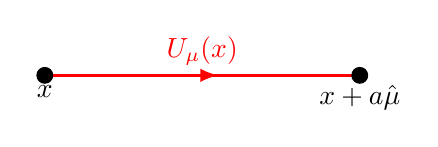
\begin{tikzpicture}
		\tikzset{middlearrow/.style={decoration={markings,mark= at position 0.55 with {\arrow{#1}} ,},postaction={decorate}}};
		\draw[middlearrow={latex}, very thick,red] (0,0)--(4,0);
		\draw[red] (2,0) node[above] {$U_{\mu}(x)$};
		\filldraw[black] (0,0) circle(0.1) node[below]{$x$};
		\filldraw[black] (4,0) circle(0.1) node[below]{$x+a\hat{\mu}$};
	\end{tikzpicture}
	\end{center}
	\caption{Link variable at point $x$ in the $\mu$ direction. $a$ is the lattice spacing.}
	\label{fig:link}
\end{subfigure}
\begin{subfigure}{0.45\textwidth}
	\begin{center}
	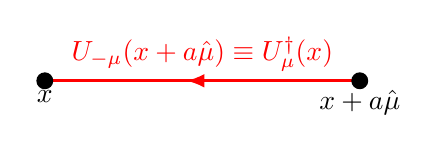
\begin{tikzpicture}
		\tikzset{middlearrow/.style={decoration={markings,mark= at position 0.55 with {\arrow{#1}} ,},postaction={decorate}}};
		\draw[middlearrow={latex}, very thick,red] (4,0)--(0,0);
		\draw[red] (2,0) node[above] {$  U_{-\mu}(x+a\hat\mu) \equiv  U^{\dagger}_{\mu}(x)$};
		\filldraw[black] (0,0) circle(0.1) node[below]{$x$};
		\filldraw[black] (4,0) circle(0.1) node[below]{$x+a\hat{\mu}$};
	\end{tikzpicture}
	\end{center}
	\caption{Link variable at point $x+a\hat\mu$ in the $-\mu$ direction.}
	\label{fig:conjg_link}
\end{subfigure}
\end{center}
\caption{Graphical representation of link variables.}
\end{figure}

Under a gauge transformation the link variables transform as
\begin{equation}
	U'_{\mu}(x) = \Omega(x) U_{\mu}(x) \Omega^{\dagger}(x+a\hat\mu),
\end{equation}
where $\Omega(x)\in\text{SU}(3)$. We refer to \cite{gattringer} for a complete discussion on lattice gauge theory.



For SU($N$), the lattice gauge action reads
\begin{equation}
	\label{eq:wilson_action}
	S[U] = \frac{\beta}{N}\sum_x \sum_{\mu < \nu} \text{Re}\ \text{Tr} \left[\mathds{1} - U_{\mu\nu}(x) \right],
\end{equation}
where $\beta = \frac{2N}{g^2}$. The plaquettes are defined by
\begin{equation}
	\label{eq:plaquette}
	U_{\mu\nu}(x) = U_{\mu}(x)U_{\nu}(x+\hat{\mu})U_{\mu}^{\dagger}(x+\hat{\nu})U_{\nu}^{\dagger}(x) 
\end{equation}

Sum of plaquette variables
\begin{equation}
	\label{eq:Sp}
	S_{\text{P}} = \frac{1}{N} \sum_x\sum_{\mu < \nu} \text{Re}\ \text{Tr} [U_{\mu\nu}(x)]
\end{equation}
we define
\begin{equation}
	\label{eq:Ep}
	E_{\text{P}} =\frac{ \langle S_{\text{P}} \rangle}{D V}
\end{equation}
where $V=L^d$ is the volume of the lattice and $D = \frac{d(d-1)}{2}$ is the number of planes of rotation.

Staples
\begin{equation}
	\label{eq:staples}
	\Sigma_{\mu}(x) = \sum_{\nu \neq \mu} \left[ U_{\nu}(x)U_{\mu}(x+\hat{\nu})U_{\nu}^{\dagger}(x+\hat{\mu}) + U_{\nu}^{\dagger}(x-\hat{\nu})U_{\mu}(x-\hat{\nu})U_{\nu}(x+\hat{\mu}-\hat{\nu})\right]
\end{equation}


The change in the action  by a local update when changing $U_{\mu}(x) \to U'_{\mu}(x)$ is
\begin{equation}
	\label{eq:DS}
	\Delta S = -\frac{\beta}{N} \text{Re } \text{Tr} \left[ \left( U'_{\mu}(x) - U_{\mu}(x) \right)\Sigma_{\mu}^{\dagger}\right]
\end{equation}

In SU(3) the SU(2) elements are of the form
\begin{equation}
\label{eq:SU2_subgroups}
	R = \begin{pmatrix}
		r_{11} & r_{12} & 0 \\
		r_{21} & r_{22} & 0 \\
		0      & 0      & 1 
	\end{pmatrix},\ S = \begin{pmatrix}
		s_{11} & 0 & s_{12} \\
		0      & 1 & 0 \\
		s_{21} & 0 & s_{22} 
	\end{pmatrix},\ T = \begin{pmatrix}
		1 & 0 & 0 \\
		0 & r_{11} & r_{12} \\
		0 & r_{21} & r_{22}
	\end{pmatrix}.
\end{equation}


	\subsection{Polyakov Loop}
	The polyakov loop is defined as the product of the link variables in the Euclidean time direction over a closed loop
	\begin{equation}
		P(\vec{x}\,) = \text{Tr}\,\prod_{t_\text{E}=1}^{L_t}U_4(\vec{x},t_\text{E}).
	\end{equation}

\subsection{Static quark potential}
One important quantity involving Polyakov loops is their correlation. The correlation function of Polyakov loops is related to the static quark potential $V(r)$ as
\begin{equation}
	\langle P(\vec{x}\,) P(\vec{y}\,)^{\dagger} \rangle \propto e^{-L_t a V(r)} \left(1 +\mathcal{O}\left( e^{-L_t a \Delta E}\right) \right),
\end{equation}
where $r = |\vec{x} - \vec{y}\,|$. Up to a constant the static quark potential is
\begin{equation}
	aV(r) = - \log(\langle P(\vec{x}\,) P(\vec{y}\,)^{\dagger} \rangle)/L_t.
\end{equation}

We use the Cornell potential to parametrize $V(r)$
\begin{equation}
	V(r) = A + \frac{B}{r} + \sigma r,
\end{equation}
here $A$ is an irrelevant additive constant, $B$ is the Coulomb part of the potential and $\sigma$ is the so called \textit{string tension}.

\section{Setting physical scales}
One method of defining a physical scale is related to the static potential. First the Sommer parameter is defined as $r_0 \approx 0.5 \ \text{fm}$, is a physical length where, roguhly speaking, the potential becomes linear.

First we compute the force 
\begin{equation}
	\label{eq:force}
	-F(r) = \frac{dV(r)}{dr} = \sigma - \frac{B}{r^2}.
\end{equation}

Using experimental data for heavy quark-antiquark pairs ($\bar{b}b$ and $\bar{c}c$) it is found that 
\begin{equation}
	-F(r_0)r_0^2 = 1.65, \ \ \ \text{where} \ \ \ r_0 \simeq 0.5 \ \text{fm}.
\end{equation}
Using the form of the force in eq.\ \eqref{eq:force} 
	\begin{equation}
		-F(r)r_0^2 = \sigma r_0^2 - B = 1.65,
	\end{equation}
which implies
	\begin{equation}
		r_0 = \sqrt{\frac{1.65+B}{\sigma}},
	\end{equation}
or in lattice units
	\begin{equation}
		\frac{r_0}{a} = \sqrt{\frac{1.65+B}{a^2\sigma}}.
	\end{equation}

The parameters $B$ and $a^2\sigma$ can be obtained by a fit to the function
\begin{equation}
	aV(an) = aA+\frac{B}{n} + a^2\sigma n,
\end{equation}	
	where $r = a n$ and $n\in \mathbb{N}$.
	Once obtained the dimensionless quantity $X = r_0/a$, the lattice spacing in physical units is $a = 0.5/X \ \text{fm}$.
	
	The temperature $T$ can be extracted by
	\begin{equation}
	\frac{1}{T}= a L_t .
\end{equation}	 
\section{Algorithms}



\subsection{Metropolis}
\begin{enumerate}
	\item Given some gauge field configuration, we go through all the lattice points in a lexicographic way. At each point $x$ in the $\mu$ direction we generate a random SU(3) matrix $U'_{\mu}(x)$.
	
	\item We compute the sum of the staples and compute the change of the action according to eq.\ \eqref{eq:DS}. We generate a uniform random number $r\in [0,1)$ and accept the change if $r \leq p$, where $p$ is
	\begin{equation}
		p = \min (1, \exp(-\Delta S)).
\end{equation}	 
\end{enumerate}

\subsection{Heatbath}
The heatbath algorithm was first implemented by Creutz for the SU(2) theory \cite{creutz1980} and generalized to SU($N$) theories by Cabbibo and Marinari \cite{cabbibo1982}. The idea for implementing the algorithm in SU($N$) is to iterate over a set of SU(2) subgroups in SU($N$) and apply the heatbath algorithm to these SU(2) elements. 

\begin{enumerate}
	\item Given some field configuration at a point $x$ and direction $\mu$, we find the sum of staples $\Sigma_{\mu}(x)$ in eq.\ \eqref{eq:staples}.
	
	\item We compute $W = U_{\mu}(x) \Sigma_{\mu}^{\dagger}(x)$ and define $W_2$ as the $2\times 2$ submatrix of $W$ that has the same block structure as $R$ (or $S$ or $T$).
	
	\item $W_2$ is a complex $2\times 2$ matrix which is generally not an element of SU(2). As described in Ref.\ \cite{kennedy1985}, we generate a matrix proportional to an SU(2) element from $W_2$ as follows
	\begin{equation}
	V = \frac{1}{2} \left[ W_2 - W_2^{\dagger} + \mathds{1}\text{Tr}\ W_2^{\dagger}\right]
	\end{equation}
	\item We compute the determinant of $V$ and take $\xi = \sqrt{\det V}$
	
	\item We follow the original heatbath implementation of Creutz. We generate a uniform random number $r \in [\exp(-\frac{4}{3}\beta \xi),1]$ and compute
	\begin{equation}
		x_0 = 1 + \frac{\log r}{\frac{2}{3}\beta \xi}.
	\end{equation}		
	
	Now we generate a uniform random number $u\in [0,1)$ and accept $x_0$ if $ u > 1 - \sqrt{1-x_0^2}$. Repeat this step until a $x_0$ is accepted.
	
	\item We now generate a vector $\vec{x} = (x_1,x_2,x_3)$ in the unit 2-sphere uniformly distributed. This may be acomplished as follows. We generate three random numbers $\vec{r} = (r_1,r_2,r_3)$ in the interval $[-1,1]$ and accept them if they are inside the unit 3-sphere. Otherwise we generate other three numbers until they are accepted. Once they are accepted we take
	\begin{equation}
		\vec{x} = \sqrt{1 - x_0^2} \frac{\vec{r}}{|\vec{r}\,|}.
	\end{equation}
	\item We have generated the elements of a SU(2) matrix $X$
	\begin{equation}
		X = \begin{pmatrix}
			x_0 + ix_1 & x_2 + ix_3 \\
		   -x_2 + ix_3 & x_0 - ix_1
		\end{pmatrix}
	\end{equation}
	\item We take
		\begin{equation}
			R_2 = X \frac{V^{\dagger}}{\xi}.
		\end{equation}
		And transform this $2\times 2$ matrix to the same block structure as the $3\times 3$ matrix $R$ (or $S$ or $T$).
		\item We go to step 2 and repeat the process to generate $S$ (or $T$) but this time taking $W = R U_{\mu}(x)\Sigma_{\mu}(x)$ (or $W = S R U_{\mu}(x)\Sigma_{\mu}(x)$).
	\item The new link element $U'_{\mu}(x)$ is
	\begin{equation}
		U'_{\mu}(x) = T S R U_{\mu}(x).
	\end{equation}			
\end{enumerate}

\section{Results}

We present simulation results for the 4-dimensional SU(3) lattice gague field theory. We implement two different local update algorithms, namely, Metropolis and Heatbath. Figure \ref{fig:Ep} shows the energy density $E_{\text{P}}$ as a function of $\beta = \frac{6}{g^2}$. There is a maximum of the slope at $5<\beta<6$, however this is not an indication of a phase transition.

\begin{center}
\begin{figure}
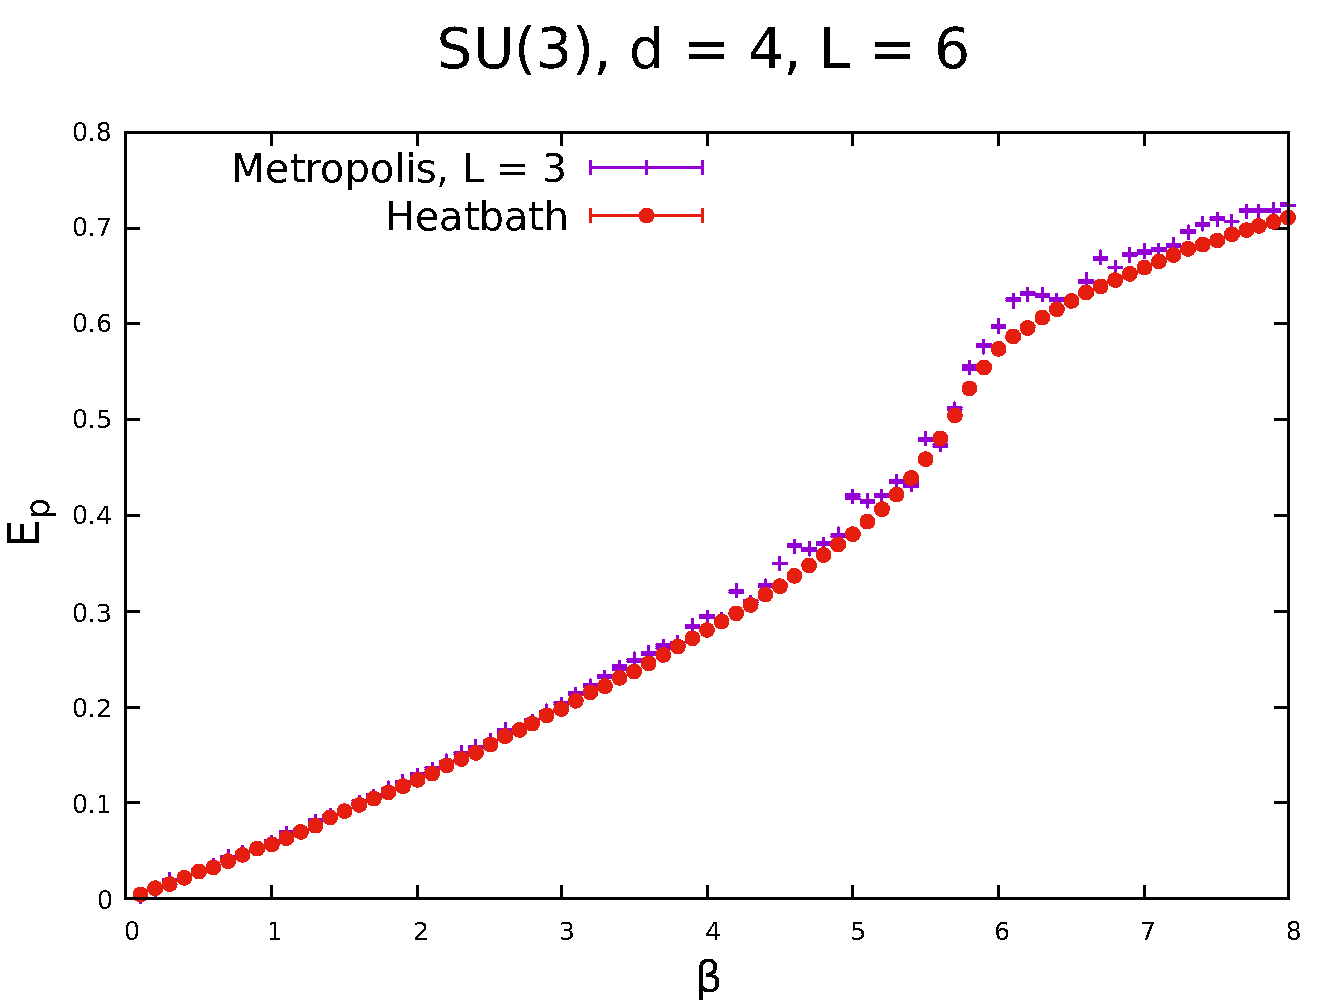
\includegraphics[scale=0.6]{../images/L=6_heatbath_L=3_metropolis.pdf}
\caption{Energy density vs. $\beta = \frac{6}{g^2}$. We simulated the SU(3) pure gauge theory in four dimensions using the Metropolis and Heatbath algorithms.}
\label{fig:Ep}
\end{figure}
\end{center}

\begin{center}
\begin{figure}
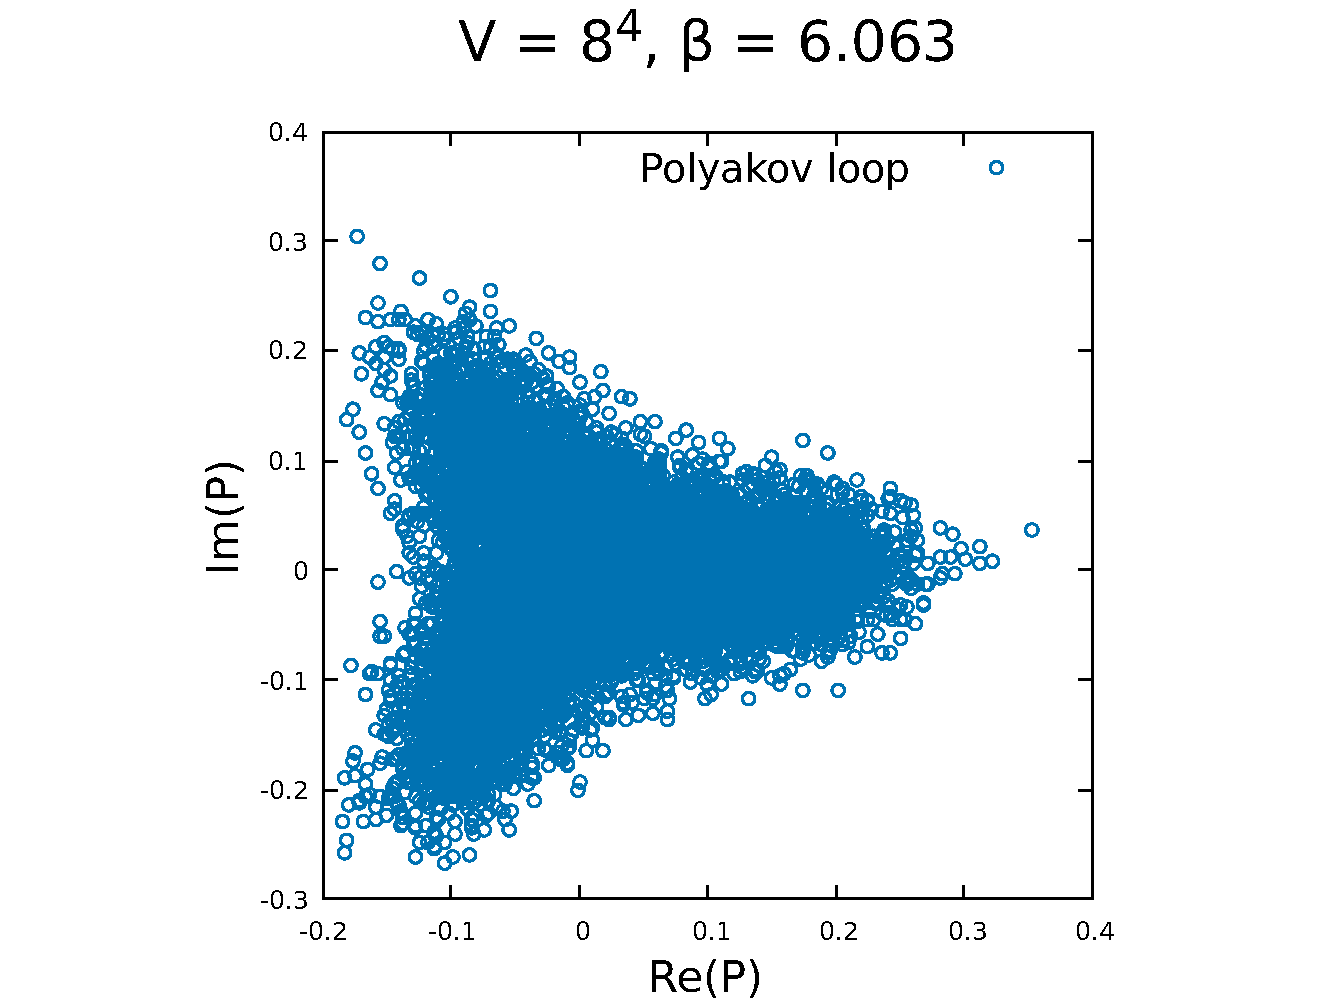
\includegraphics[scale=0.6]{../images/polyakov_loop.pdf}
\caption{Scatter plot of the expectation value of the Polyakov loop at $\beta = 6.063$ and volume $V = 8^4$.}
\label{fig:poly}
\end{figure}
\end{center}

\begin{center}
\begin{figure}
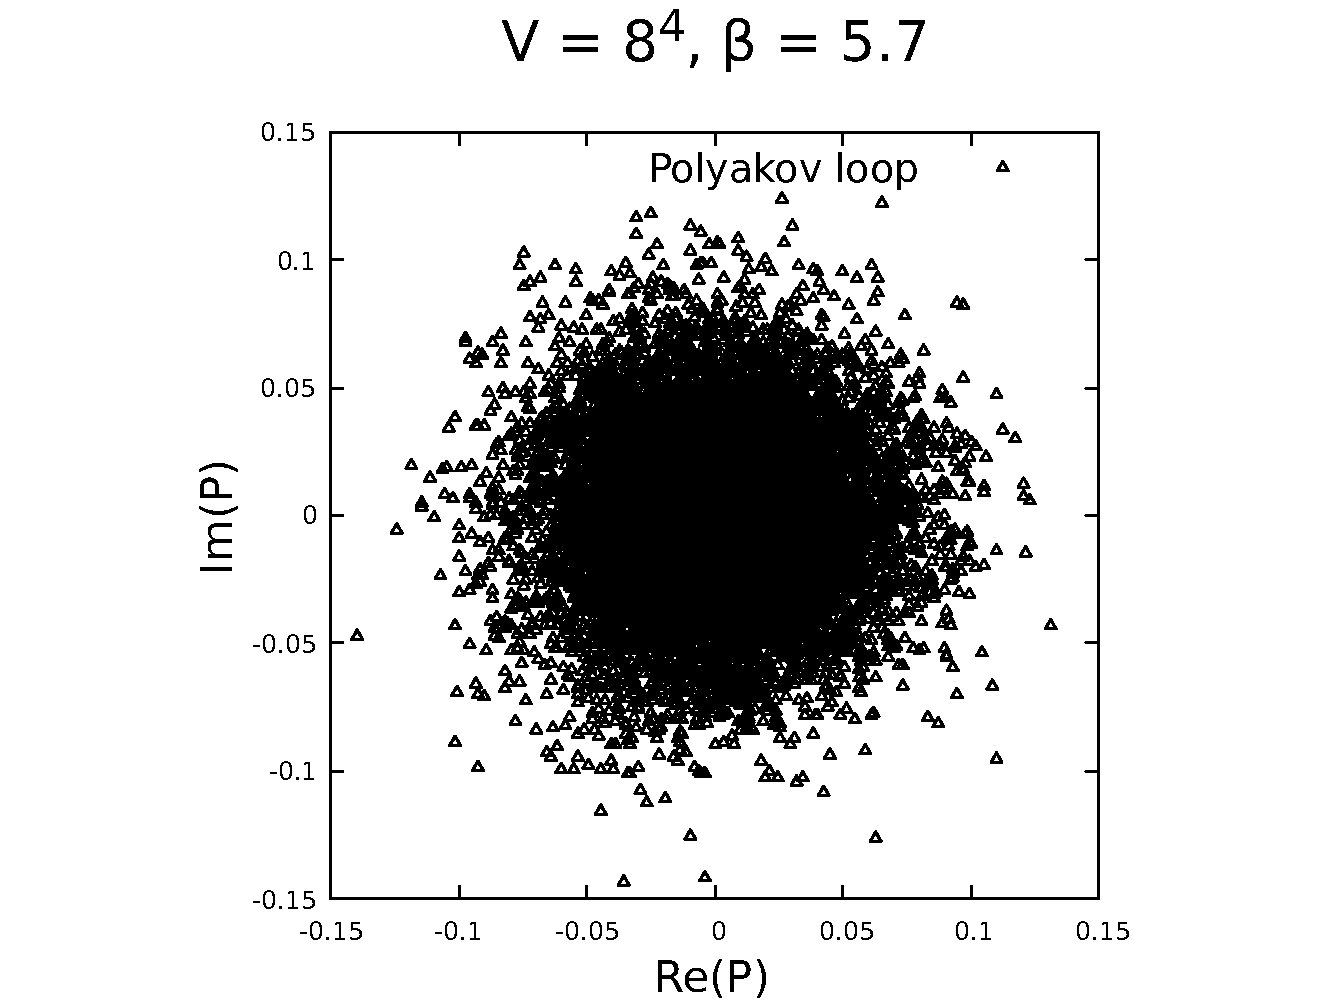
\includegraphics[scale=0.6]{../images/polyakov_loop_beta=57.pdf}
\caption{Scatter plot of the expectation value of the Polyakov loop at $\beta = 5.7$ and volume $V = 8^4$.}
\label{fig:poly}
\end{figure}
\end{center}


With a volume $16^3 \times 6$ and at $\beta = 5.7$ the static potential $aV(an)$ using the correlation of the Polyakov loop is seen in figure \ref{fig:correlation_polyakov}. We obtained a string tension $a^2\sigma = 0.042$ and $B = -0.49$, therefore
\begin{equation}
	\frac{r_0}{a} = \sqrt{\frac{1.65 - 0.49}{0.042}} = 5.25,
\end{equation}
and the lattice spacing in physical units corresponds to
\begin{equation}
	a = 0.5/ 5.25 \ \text{fm} = 0.095 \ \text{fm}.
\end{equation}
Finally the temperature corresponds to $T = \frac{197 \ \text{MeV}}{aL_t}  = \frac{197\ \text{MeV}}{0.095 \cdot 6} = 345 \ \text{MeV}$.
\begin{figure}
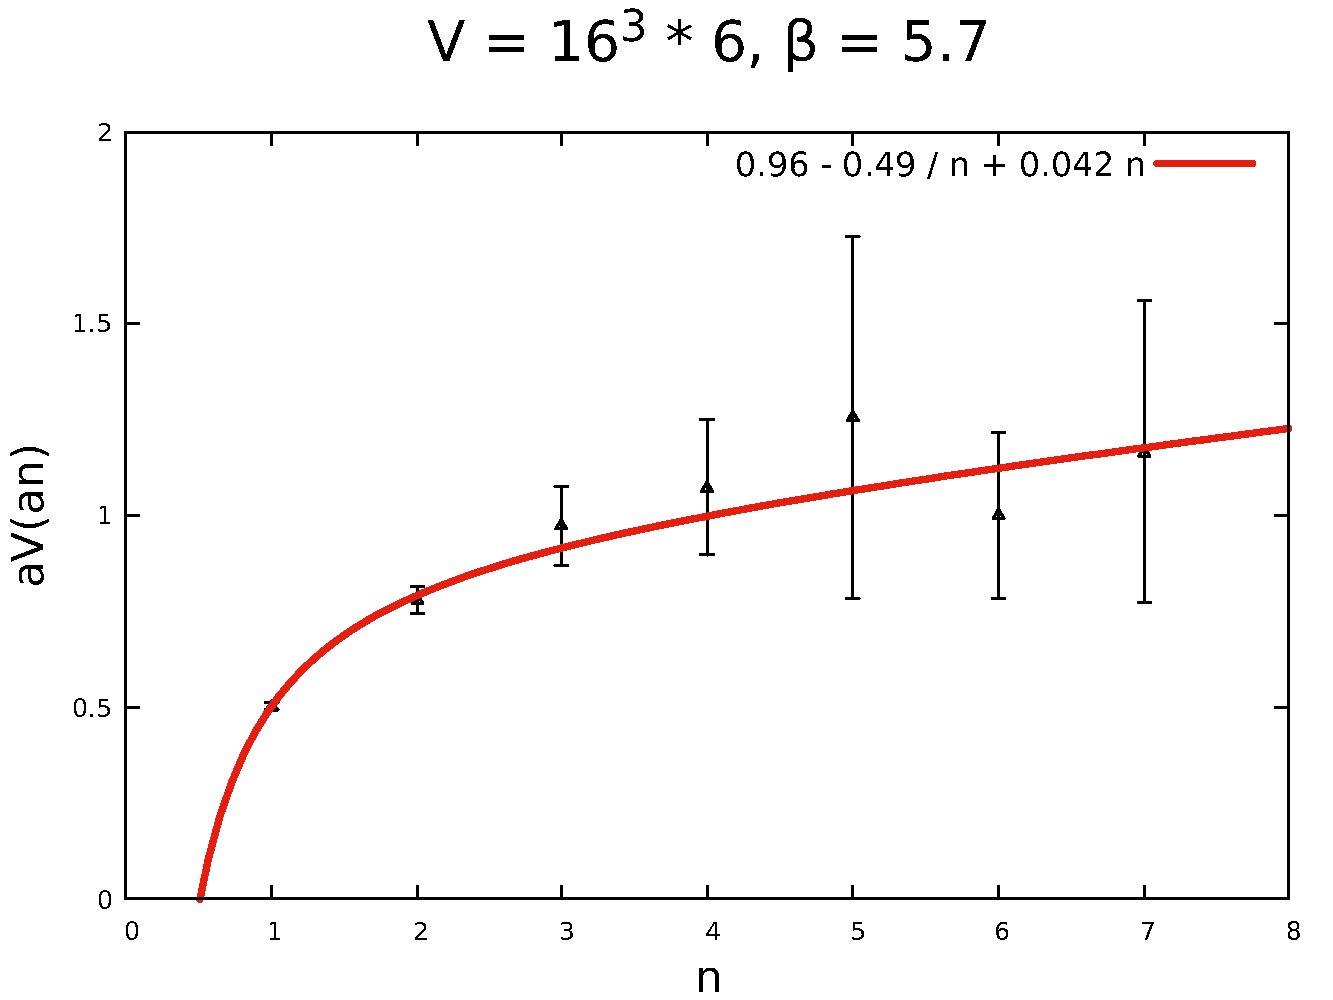
\includegraphics[scale=0.6]{../images/correlation_polyakov.pdf}
\caption{Static quark potential.}
\label{fig:correlation_polyakov}
\end{figure}
\section{Acknowledgements}
The author thanks Dr.\ Wolfgang Bietenholz for funding (in the form of meals) this research. Thanks to Dr.\ Urs Gerber for providing a recipe for implementing the heatbath algorithm for the U(1) gauge theory at an early stage of this research. Finally, I want to thank Ariana Grande, The Weeknd and Polyphia for giving the right inspiration while working on this paper. Without their music I could have easily gone crazy.


\begin{thebibliography}{99}

\bibitem{gattringer} C.\ Gattringer and C.B.\ Lang, \emph{Quantum Chromodynamics on the Lattice: An Introductory Presentation},  Lect.\ Notes Phys.\ 788 (Springer, Berlin Heidelberg 2010).

\bibitem{Metropolis} N.\ Metropolis {\it et al.},
\emph{Equation of State Calculations by Fast Computing Machines},
J.\ Chem.\ Phys.\ {\bf 21} (1953) 1087.

\bibitem{Glauber} R.J.\ Glauber,
  \emph{Time-Dependent Statistics of the Ising Model},
  J.\ Math.\ Phys.\ {\bf 4} (1963) 294.
  
\bibitem{Gerber} U.\ Gerber,
  \emph{Heatbath Algorithm for the 2d U(1) Model}.
  Informal Notes. Universidad Nacional Autónoma de México, 2015.  
  
  \bibitem{creutz1980} M. Creutz, \emph{Monte Carlo Study of the Quantized SU(2) Gauge Theory.} Phys.\ Rev.\ D {\bf 21} (1980) 2308-2315.

\bibitem{cabbibo1982} N. Cabbibo, E. Marinari, \emph{A New Method for Updating SU(N) Matrices in Computer Simulations of Gauge Theories}, Phys.\ Lett.\ B {\bf 119} (1982) 387-390.

\bibitem{kennedy1985} A.D.\ Kennedy, B.J.\ Pendleton, \emph{Improved Heatbath Method for Monte Carlo Calculations in Lattice Gauge Theories}, Phys.\ Lett.\ {\bf 156B} (1985) 393-399.
\end{thebibliography}

\end{document}